\documentclass[12pt,a4paper]{article}

\usepackage[utf8]{inputenc}
\usepackage{graphicx}
\usepackage{geometry}
\usepackage{setspace}
\usepackage{booktabs}
\usepackage{hyperref}
\usepackage{caption}

\geometry{top=1.8cm, bottom=1.8cm, left=2cm, right=2cm}
\setstretch{0.88}
\parskip=2pt
\parindent=0pt
\small

\title{\textbf{Laporan Tugas Autoencoder}\\[4pt]
\large Training di Kaggle dan Rekonstruksi Citra Fashion-MNIST melalui Decoder}
\author{Nama: Fatih Jawwad Al Mumtaz \\ NIM: 452024611047}
\date{}

\begin{document}

\maketitle
\thispagestyle{empty}
\newpage

\section{Arsitektur Autoencoder}

Autoencoder adalah jaringan saraf tiruan yang terdiri atas dua komponen utama, yaitu encoder dan decoder. Encoder berperan mereduksi dimensi citra input menjadi representasi laten (latent vector) yang berisi fitur-fitur esensial dari citra. Decoder kemudian membangun kembali citra dari representasi laten tersebut menuju bentuk aslinya. Arsitektur yang digunakan dalam tugas ini disusun secara simetris. Encoder terdiri atas dua lapisan konvolusi dengan masing-masing 16 dan 32 filter, diikuti oleh lapisan fully connected yang memetakan fitur ke latent space. Decoder menyusun ulang citra melalui lapisan fully connected dan dua lapisan transposed convolution yang mengembalikan dimensi asli 28×28 piksel. Fungsi aktivasi ReLU digunakan pada setiap lapisan tersembunyi, sementara sigmoid digunakan pada output decoder untuk menghasilkan nilai piksel dalam rentang 0 hingga 1.

\section{Proses Training di Kaggle}

Training dilakukan menggunakan Kaggle Notebook dengan dataset Fashion-MNIST yang terdiri atas 60.000 citra pelatihan dan 10.000 citra pengujian berukuran 28×28 piksel grayscale. Model dilatih menggunakan loss function Mean Squared Error (MSE) dan optimizer Adam dengan learning rate 0,001. Untuk mempelajari pengaruh ukuran latent space terhadap kualitas rekonstruksi, dilakukan eksperimen pada tiga variasi latent dimension, yaitu 2, 8, dan 32. Masing-masing model dilatih selama 20 epoch hingga nilai loss konvergen. Selama proses training, grafik loss dicatat dan divisualisasikan untuk memantau konvergensi. Setelah training selesai, model disimpan dalam format .pth dan diunduh dari Kaggle untuk digunakan pada proses inferensi di lingkungan lokal.

\section{Hasil Eksperimen}

\subsection{Grafik Training Loss}

Gambar 1 menunjukkan perbandingan training loss dari ketiga variasi latent dimension. Terlihat bahwa latent dimension yang lebih besar cenderung menghasilkan loss yang lebih rendah karena kapasitas representasi yang lebih besar.

\begin{figure}[!ht]
\centering
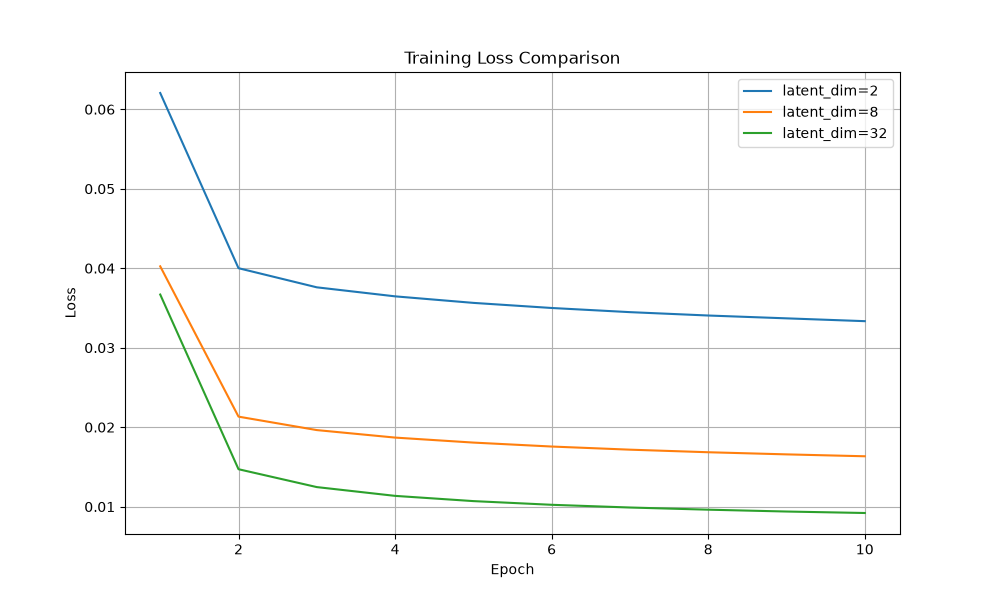
\includegraphics[width=0.75\textwidth]{results/training_loss_comparison.png}
\caption{Perbandingan training loss antar latent dimension}\vspace{-8pt}
\end{figure}

\subsection{Perbandingan Hasil Rekonstruksi}

Gambar 2 menampilkan perbandingan citra asli dengan hasil rekonstruksi untuk setiap ukuran latent dimension pada empat sampel data uji.

\begin{figure}[!ht]
\centering
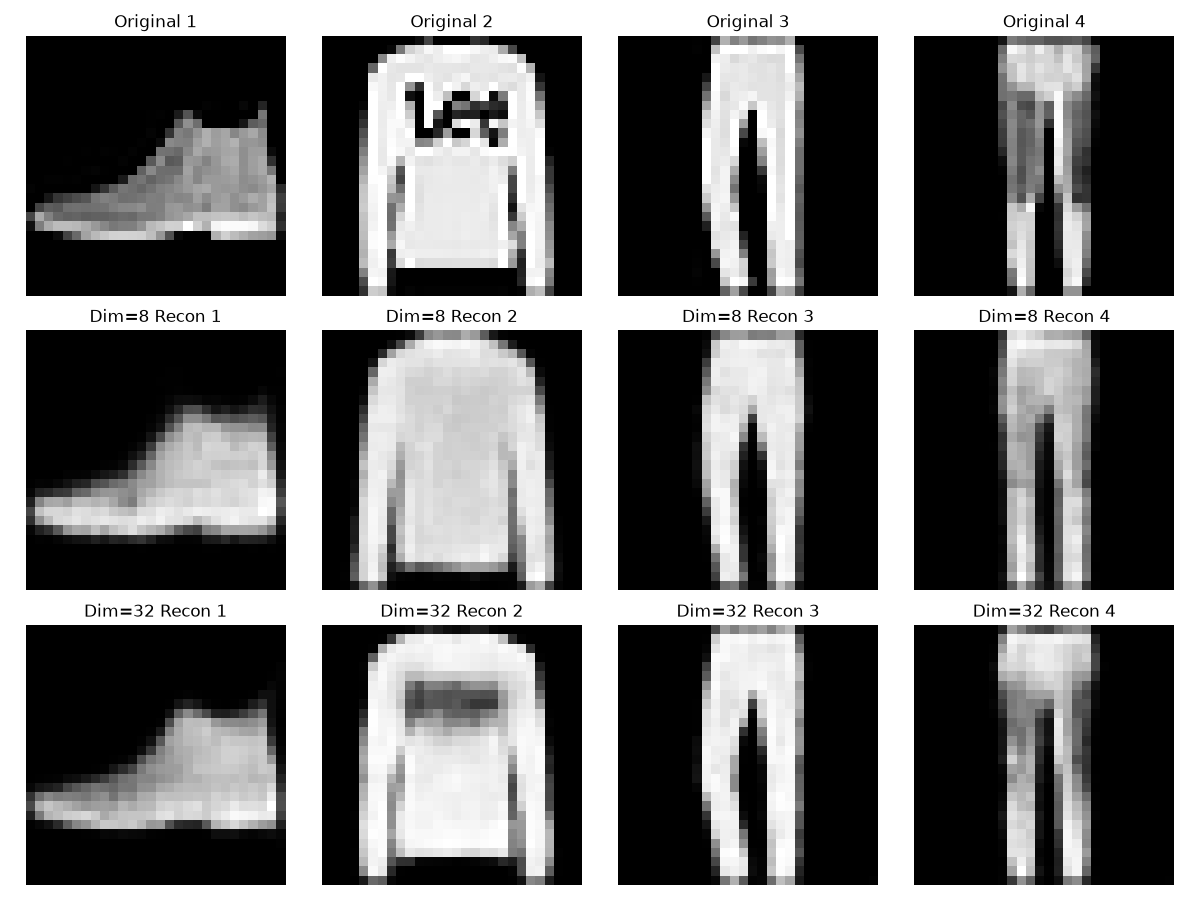
\includegraphics[width=0.82\textwidth]{results/reconstruction_comparison.png}
\caption{Perbandingan rekonstruksi antar latent dimension}
\end{figure}

\subsection{Tabel Perbandingan}

\begin{table}[!ht]
\centering
\caption{Perbandingan hasil eksperimen antar latent dimension}
\begin{tabular}{cccc}
\toprule
Latent Dim & Loss Akhir & Kualitas Visual & Catatan \\
\midrule
2 & 0,0325 & Buram, tepi tidak jelas, bentuk sulit dikenali & Kapasitas representasi sangat terbatas \\
8 & 0,0151 & Cukup jelas, detail tepi mulai terbentuk & Keseimbangan antara kompresi dan detail \\
32 & 0,0081 & Paling tajam, detail hampir mendekati asli & Rekonstruksi terbaik \\
\bottomrule
\end{tabular}
\end{table}

\section{Rekonstruksi Melalui Terminal}

Proses rekonstruksi dilakukan melalui terminal menggunakan dua program Python, yaitu \texttt{reconstruct.py} untuk rekonstruksi dengan autoencoder penuh dan \texttt{generate\_from\_decoder.py} untuk generasi citra dari decoder saja.

\subsection{Rekonstruksi dengan Autoencoder Penuh}

Perintah berikut digunakan untuk merekonstruksi citra Fashion-MNIST pada indeks tertentu:

{\footnotesize\begin{verbatim}
python reconstruct.py --model models/autoencoder_fashion_mnist_dim32.pth
    --latent_dim 32 --index 25 --outdir results
\end{verbatim}}

Program akan menghasilkan tiga file: \texttt{original.png}, \texttt{reconstructed.png}, dan \texttt{comparison.png}.

\subsection{Generasi Citra dari Decoder}

Decoder dapat digunakan secara mandiri untuk menghasilkan citra dari latent vector yang diberikan. Untuk latent dimension 2:

{\footnotesize\begin{verbatim}
python generate_from_decoder.py --decoder models/decoder_fashion_mnist_dim2.pth
    --latent_dim 2 --z1 0.5 --z2 -1.2
\end{verbatim}}

Untuk latent dimension lebih besar, digunakan argumen \texttt{--latent}:

{\footnotesize\begin{verbatim}
python generate_from_decoder.py --decoder models/decoder_fashion_mnist_dim8.pth
    --latent_dim 8 --latent "0.5,-1.2,0.3,0.8,0.1,-0.5,0.7,1.0"
\end{verbatim}}

\subsection{Screenshot Terminal}

\begin{figure}[!ht]
\centering
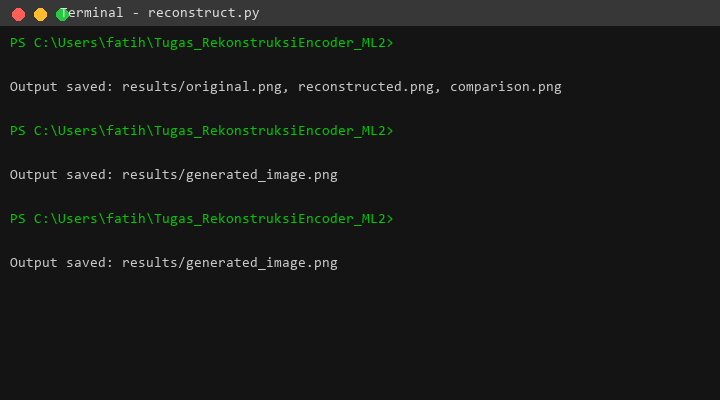
\includegraphics[width=0.75\textwidth]{results/terminal_screenshot.png}
\caption{Screenshot proses rekonstruksi melalui terminal}
\end{figure}

\section{Analisis}

Pada model autoencoder, encoder berperan sebagai komponen yang mereduksi citra Fashion-MNIST dari dimensi 28×28 piksel menjadi representasi laten berdimensi lebih kecil. Representasi ini menyimpan informasi penting dari objek dalam citra, seperti pola umum, kontur, dan struktur visual dari berbagai jenis pakaian. Proses reduksi ini bekerja melalui lapisan konvolusi yang mengekstrak fitur hierarkis, mulai dari tepi sederhana hingga pola yang lebih kompleks. Informasi yang telah dikompresi dalam bentuk latent vector kemudian menjadi satu-satunya sumber bagi decoder untuk membangun kembali citra. Hal ini berarti kualitas rekonstruksi sangat bergantung pada seberapa baik latent vector mampu menangkap informasi esensial dari citra asli.

Decoder berperan sebagai kebalikan dari encoder, yaitu mengubah representasi laten kembali menjadi citra berdimensi penuh. Melalui lapisan transposed convolution, decoder menyusun ulang pola-pola visual dari fitur yang telah diekstrak oleh encoder. Proses ini menunjukkan bahwa decoder tidak bekerja secara arbitrer, melainkan telah mempelajari pemetaan dari latent space ke ruang citra selama pelatihan. Ketika decoder diberikan latent vector acak, citra yang dihasilkan masih menyerupai pakaian Fashion-MNIST meskipun tidak identik dengan data pelatihan mana pun. Ini membuktikan bahwa decoder telah mempelajari distribusi data secara statistik, bukan sekadar menyalin input.

Latent space merupakan ruang representasi fitur berdimensi rendah tempat encoder memproyeksikan citra input. Makna dari latent space adalah bahwa titik-titik dalam ruang ini merepresentasikan variasi fitur dalam data, seperti jenis pakaian, orientasi, dan ketebalan. Jarak antar titik dalam latent space mencerminkan kemiripan visual antar citra. Semakin besar latent dimension, semakin banyak derajat kebebasan yang dimiliki model untuk merepresentasikan variasi tersebut. Namun, latent space yang terlalu besar juga berpotensi menyimpan informasi redundan atau noise.

Pengaruh latent dimension terhadap kualitas rekonstruksi terlihat jelas dari hasil eksperimen. Pada latent dimension 2, model harus mengompresi seluruh informasi citra ke dalam hanya dua bilangan, sehingga banyak detail yang hilang. Hasil rekonstruksi tampak buram dan bentuk pakaian sulit dibedakan secara jelas. Pada latent dimension 8, kualitas rekonstruksi meningkat secara signifikan. Detail tepi mulai terbentuk dan struktur objek lebih mudah dikenali. Pada latent dimension 32, kualitas rekonstruksi paling baik dengan detail yang hampir mendekati citra asli.

Hubungan antara nilai loss dan kualitas visual menunjukkan bahwa loss yang lebih rendah secara umum berkorelasi dengan hasil visual yang lebih baik. Akan tetapi, penurunan loss tidak selalu linear dengan peningkatan kualitas visual yang dirasakan. Perbedaan antara latent dimension 8 dan 32 dalam metrik loss cukup signifikan, tetapi secara visual perbaikannya mungkin tidak setajam perbedaan antara latent dimension 2 dan 8. Hal ini menunjukkan bahwa pada titik tertentu, penambahan kapasitas latent space memberikan pengembalian yang semakin berkurang terhadap kualitas visual.

Proses rekonstruksi melalui terminal memiliki perbedaan mendasar dengan rekonstruksi di dalam notebook. Pada notebook, seluruh proses mulai dari inisialisasi model, loading dataset, hingga inferensi dilakukan dalam satu lingkungan yang sama. Pada terminal, model harus disimpan terlebih dahulu sebagai file .pth, kemudian dimuat ulang dalam program Python terpisah. Hal ini menuntut kesesuaian arsitektur model yang persis sama antara saat training dan inferensi. Ketidakcocokan arsitektur, seperti perbedaan jumlah neuron pada lapisan fully connected, akan menyebabkan kegagalan saat memuat parameter model. Selain itu, program terminal juga harus mengimpor definisi arsitektur yang identik dengan yang digunakan saat training.

Decoder membutuhkan latent vector sebagai input karena decoder tidak memiliki akses langsung ke citra asli. Seluruh informasi yang dimiliki decoder tentang citra yang akan dihasilkan berasal dari latent vector yang diberikan. Ketika decoder digunakan secara mandiri dengan latent vector acak, kualitas citra yang dihasilkan bervariasi. Beberapa latent vector menghasilkan citra yang tampak seperti pakaian yang realistis, sementara yang lain menghasilkan bentuk yang tidak jelas. Hal ini menegaskan bahwa decoder hanya mampu menavigasi ruang citra yang telah dipelajari dari distribusi data pelatihan.

Refleksi kritis terhadap hasil eksperimen menunjukkan bahwa autoencoder tidak sepenuhnya memahami struktur gambar secara semantik. Autoencoder belajar merekonstruksi citra dengan meminimalkan perbedaan piksel demi piksel antara input dan output, bukan dengan memahami bahwa objek yang direkonstruksi adalah pakaian. Namun, melalui proses training pada ribuan citra, autoencoder secara implisit mempelajari pola statistik yang umum dalam data Fashion-MNIST, seperti simetri, kontur, dan tekstur. Hal ini terbukti dari kemampuan decoder menghasilkan citra yang masuk akal dari latent vector acak, yang menunjukkan bahwa model telah menangkap distribusi data, bukan sekadar menghafal pola piksel.

\section{Kesimpulan}

Berdasarkan hasil eksperimen, dapat disimpulkan bahwa autoencoder mampu merekonstruksi citra Fashion-MNIST dengan kualitas yang bervariasi tergantung pada ukuran latent dimension. Latent dimension yang lebih besar menghasilkan rekonstruksi yang lebih baik karena kapasitas representasi yang lebih besar, namun meningkatkan risiko overfitting dan penggunaan memori yang lebih tinggi. Model autoencoder yang telah dilatih dapat digunakan kembali melalui terminal dengan cara menyimpan dan memuat ulang parameter model. Proses rekonstruksi melalui decoder secara mandiri membuktikan bahwa decoder telah mempelajari pemetaan dari latent space ke ruang citra. Autoencoder tidak memahami gambar secara semantik, melainkan mempelajari pola statistik dari data pelatihan untuk meminimalkan kesalahan rekonstruksi.

\end{document}
